\chapter[Product]{Design and Implementation}
\label{design}

	\section{Introduction}
	\label{design:intro}

		Due to the room for research available in this area, it made sense to focus this study on a relatively broad area of the subject to be used as a foundation, rather than to specialise on a particular niche.
		Because of this, the main focus for this study is the effects that Non-Euclidean geometry has on a user's sense of Immersion, and to find any changes in a user's comfort navigating in a virtual environment.

		This chapter covers the development process that was undertaken for the creation of the product used for the experiments.

	\section{Development Processes}
	\label{design:dev}

		Before development on the system could begin, the tools which were to be used for the system needed to be chosen.

		Unity v5.3.4f1 \cite{UnityTechnologies2016} was chosen for the development of the system to be used in the study.
		The Unity engine was used as the base for the product due to its existing compatibility with the VR system to be used during the experiments, as well as the fact that due to its inclusion of optimised rendering systems other required features of a game engine, work on the product could focus specifically on the unique features required for the system \cite{Bruce2012}.
		As well as this, the 0.1.3.0-beta version of the \enquote{Oculus Utilities for Unity 5} \cite{Oculus2016} was included, to ensure the system had maximum compatibility with the Oculus Rift DK2 that was to be used with it.
		Using this would ensure that the motion tracking of the user would be calibrated correctly for the hardware, avoiding sensorimotor maladaptation from occurring from prolonged exposure to the virtual environment \cite{Wright2014}.
		The navigation within game scenes was done using the \enquote{OVRPlayerController} included with the Oculus Utilities.

		As a way to manage the project during its development, the Git version control system was used, with the repository hosted by GitHub.
		By using a version control system such as Git, there would always be a complete, fully revertible change history for the project during development.
		This ensures that if functionality of the system was ever broken, and the reason for it is unclear, files can be reverted to previous working states with ease.
		As well as this, using git's branch system, multiple potentially breaking features of the product can be developed separately from each other, and simultaneously, by switching between the active branches.
		This allows for fast, iterative prototyping on the implementation of the system during its development.
		Finally, the fact that all required files for the system were being hosted remotely on the git repository server, the project would never be at risk of being lost due to local hardware failure.

	\section[Implementation]{Product Implementation}
	\label{design:model}

		To achieve the effect that a player is inside a non-Euclidean environment, a total of three primary pieces of functionality needed to be implemented:
		\begin{enumerate}
			\item A way to position a camera in a way to get the perspective of an area which would be seen by the player of the area which would give the impression of non-Euclidean space
			\item A way to render the new perspective to be seen by the player, but only in desired areas
			\item A way to transport the player between their current position and the new perspective without them realising they have gone anywhere other than they expected.
		\end{enumerate}

		To calculate the relative position for a camera to render a new perspective for the player, two pieces of information needed to be known: the plane where the player would be viewing the perspective from (hereby referenced as \enquote{from plane}), and a plane in the new area that the player would be viewing the perspective of (hereby referenced as \enquote{to plane}) (Note that \enquote{plane} is being used in this context as an area reference. Any object type could be used for the viewing areas in the completed system).
		Both planes can be seen referenced by the two \enquote{View Area} lines in \autoref{design:fig:maths}.

		With the two relative points known, the next step is to work out the positioning and rotation that the camera will need to use for the new area.
		The position of the camera could be worked out by calculating the distance vector between the player and the \enquote{from plane}, represented by \enquote{A} (Z axis) and \enquote{B} (X Axis) on \autoref{design:fig:maths}, with an unseen \enquote{C} which would represent the distance in the Y axis.
		The position offset then needs to be reoriented by the difference in rotation between the \enquote{from plane} and \enquote{to plane}, before finally being translated relative to the position of the \enquote{to plane}.
		This calculation can be seen in lines 90 or 93 in \autoref{appendix:code:camera}.

		\begin{figure}[h]
			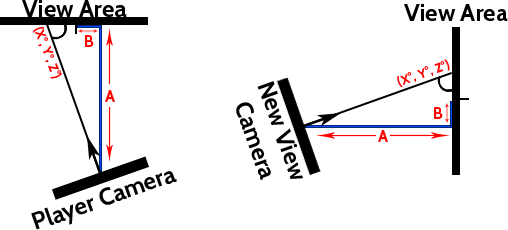
\includegraphics[width=1\textwidth]{Images/Position}
			\centering
			\caption{Top-down 2D representation of the calculations for the position and rotation of cameras.
				See \autoref{appendix:code:camera} for the implementation}
			\label{design:fig:maths}
		\end{figure}

		The next step was to calculate the rotation to use for the camera.
		In order to find out the rotation that is needed for the camera, two calculations needed to be made.
		The first is one which was done before, which is the difference in rotation between the \enquote{from plane} and the \enquote{to plane}.
		The second is the difference in rotation between the player camera, and the normal of the \enquote{from plane} (Represented by \enquote{(X\degree, Y\degree, Z\degree)} in \autoref{design:fig:maths}).
		With these two rotations known, the final rotation of the perspective camera can be calculated.
		This calculation can be seen in lines 91 or 94 in \autoref{appendix:code:camera}.

		One of the more challenging aspects for achieving the non-Euclidean effect in the scene was getting the new perspective camera to render appropriately in the scene itself.
		The usual approach for rendering different views in Unity is to use their provided \enquote{Render Textures}, which allow you to render a camera to a texture, and use that as the texture of an object in the game world.
		Although that method works well for regular games outside of VR for things like mirrors, it was not a valid solution for use in VR where the user can perceive depth in the virtual environment, due to the texture being rendered on a flat mesh.

		To get around this issue, a custom shader was made (\autoref{appendix:code:shader}) which could be applied to an object which was acting as the area for where a user should see the new perspective.
		This shader had three main features: it would write the position of the object to the Z buffer for the render queue to ensure nothing behind it would be rendered, it would write no data to the RGBA (colour) channels to ensure nothing would be visibly rendered in that position from the player's perspective, and finally it would always be the last thing to be rendered in the scene (Other than UI elements) to ensure the area would always be clear.
		An object with the shader in use can be seen in \autoref{design:fig:cullview}.

		\begin{figure}[h]
			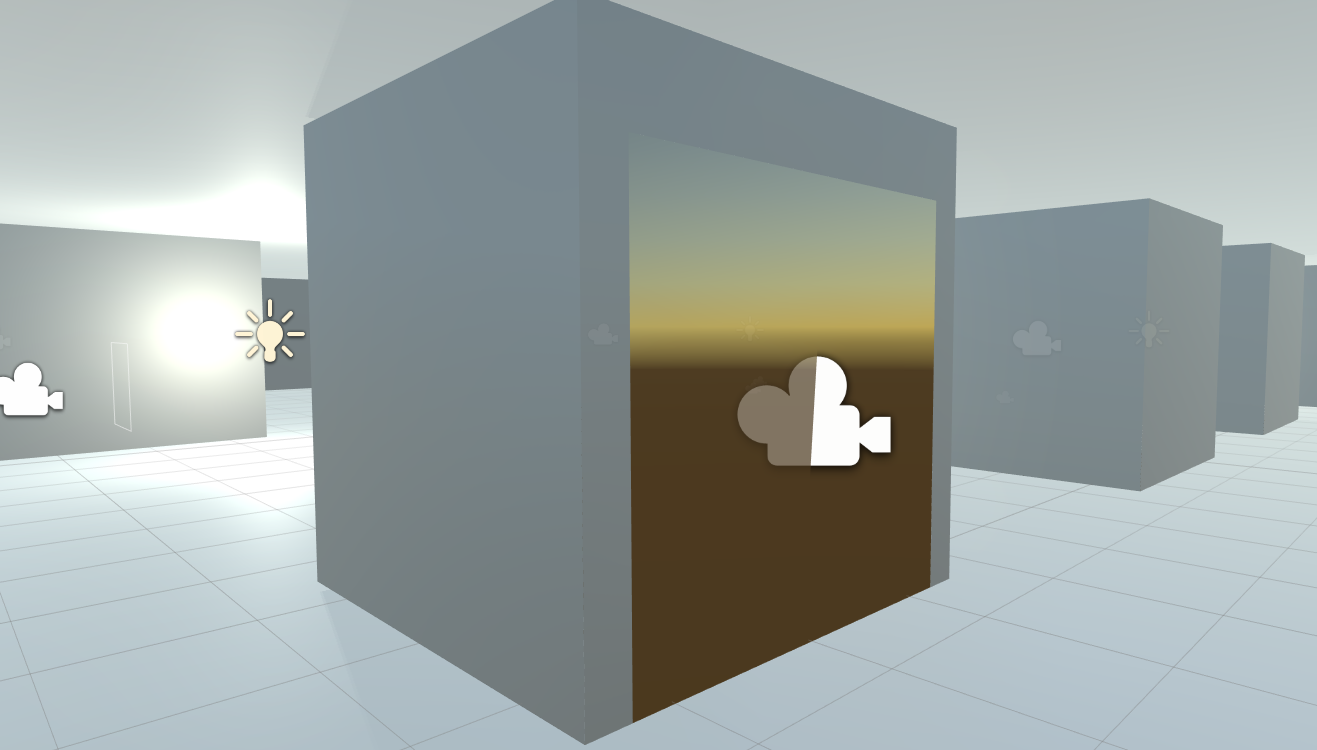
\includegraphics[width=1\textwidth]{Images/NE_Scene_View}
			\centering
			\caption{Example of view of the culling shader before the new view is rendered. The brown gradient texture scene in the rectangle is the skybox for the scene}
			\label{design:fig:cullview}
		\end{figure}

		\begin{figure}[h]
			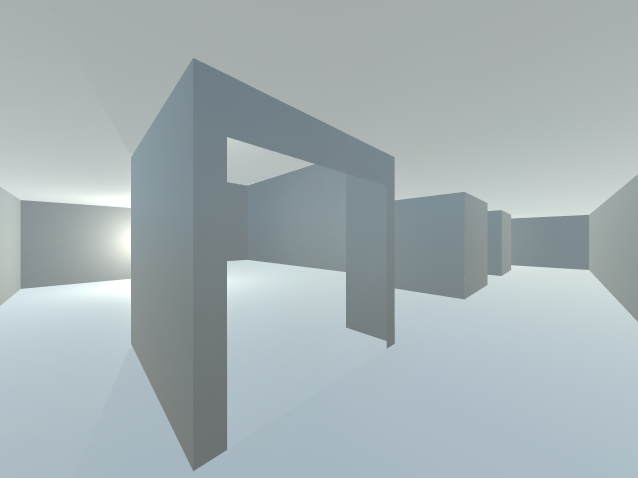
\includegraphics[width=1\textwidth]{Images/NE_View}
			\centering
			\caption{Example of view of the final effect inside the Non-Euclidean scene, displaying an area which appears larger than the container surrounding it}
			\label{design:fig:game}
		\end{figure}

		With objects placed in the scene with the shader, it would allow the view from the new perspective cameras, which had their own render queues so the effect would not overwrite them, to be drawn in place of those objects.
		When coupled with the correct positioning and rotations of the perspective camera, it gave the impression that the other perspective was directly in those areas, in full stereoscopic 3D (As seen in \autoref{design:fig:game}).

		With the illusion working visibly, the final step was to allow the user to navigate between the areas in a way that gives no indication to the user that they have been transported.
		The calculations for the actual positioning of the player once being transported were similar to that of the perspective camera positioning, where it would calculate a position for the player, and a rotation for the camera, relative to the \enquote{from plane} and \enquote{to plane} (\autoref{appendix:code:player}).
		The next calculation which needed to be done for the player positioning was to know when to transport the player.
		To do this, a collision area was added to the \enquote{from plane} and \enquote{to plane} objects.
		In the collision areas, instead of stopping the player from moving within them, they would be used to detect if the player has moved greater than half way through the area, and if so, they would be transported to the equivalent area in the connected plane (\autoref{appendix:code:player}, line 142).
		From here, the only additional calculation that needed to be made was to adjust the vector containing the player's movement momentum, and adjust it to be relative to the rotation offset between the two planes.
		To do this, the movement vector for the player needed the same rotation applied that was made to the player's orientation.

		As a way of assisting with the modelling of the scenes themselves, lines were drawn inside the scene views of the Unity editor which would symbolise the various aspects of the connected points (\autoref{design:fig:scene}).
		In the figure, red lines indicate the locations of the \enquote{from plane} and \enquote{to plane} for the connections, green lines indicate the normals of the planes, and yellow lines indicate planes which are visible to the player at any given time.
		Only planes which are currently visible by the player have their respective perspective cameras positioned and rendered.

		\begin{figure}[H]
			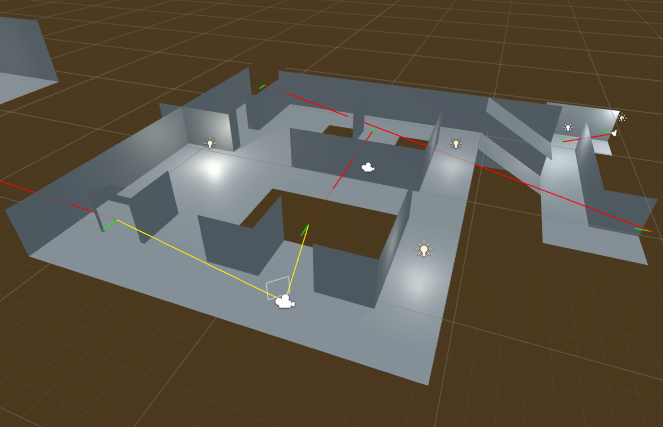
\includegraphics[width=1\textwidth]{Images/Lines_Everywhere2}
			\centering
			\caption{Example view of a scene in the Unity editor.}
			\label{design:fig:scene}
		\end{figure}

	\section[Environment Design]{Design of experiment environments}
	\label{design:design}

		The design of the environments to be used in the experiments is almost as important as the functionality of the system itself, as it is the only medium through which the participants will be able to provide feedback.
		Two separate scenes were created for use in the experiments, one where the participants would be navigating through a non-Euclidean environment, and the other which would only make use of standard Euclidean space.

		To limit the number of factors which could affect the immersion of a participant in the experiments, a minimalistic aesthetic was chosen for the scenes.
		By using simple white texturing and relying on lighting for definition, impurities that could be noticed by pixelation of detailed textures were removed, focusing the participant's attention solely on the geometry of the scenes.
		Similarly, the scenes themselves were modelled using simple primitive shapes, such as planes and cubes, to try and minimise any impacts in immersion that could be caused by low polygon counts in more complex models.
		Testing was done on scenes which used more detailed textures (\autoref{design:fig:design:tex}), however any imperfections in the scene were much more apparent in this scene compared to the minimalistic designs of the completed experiment scenes.

		\begin{figure}[H]
			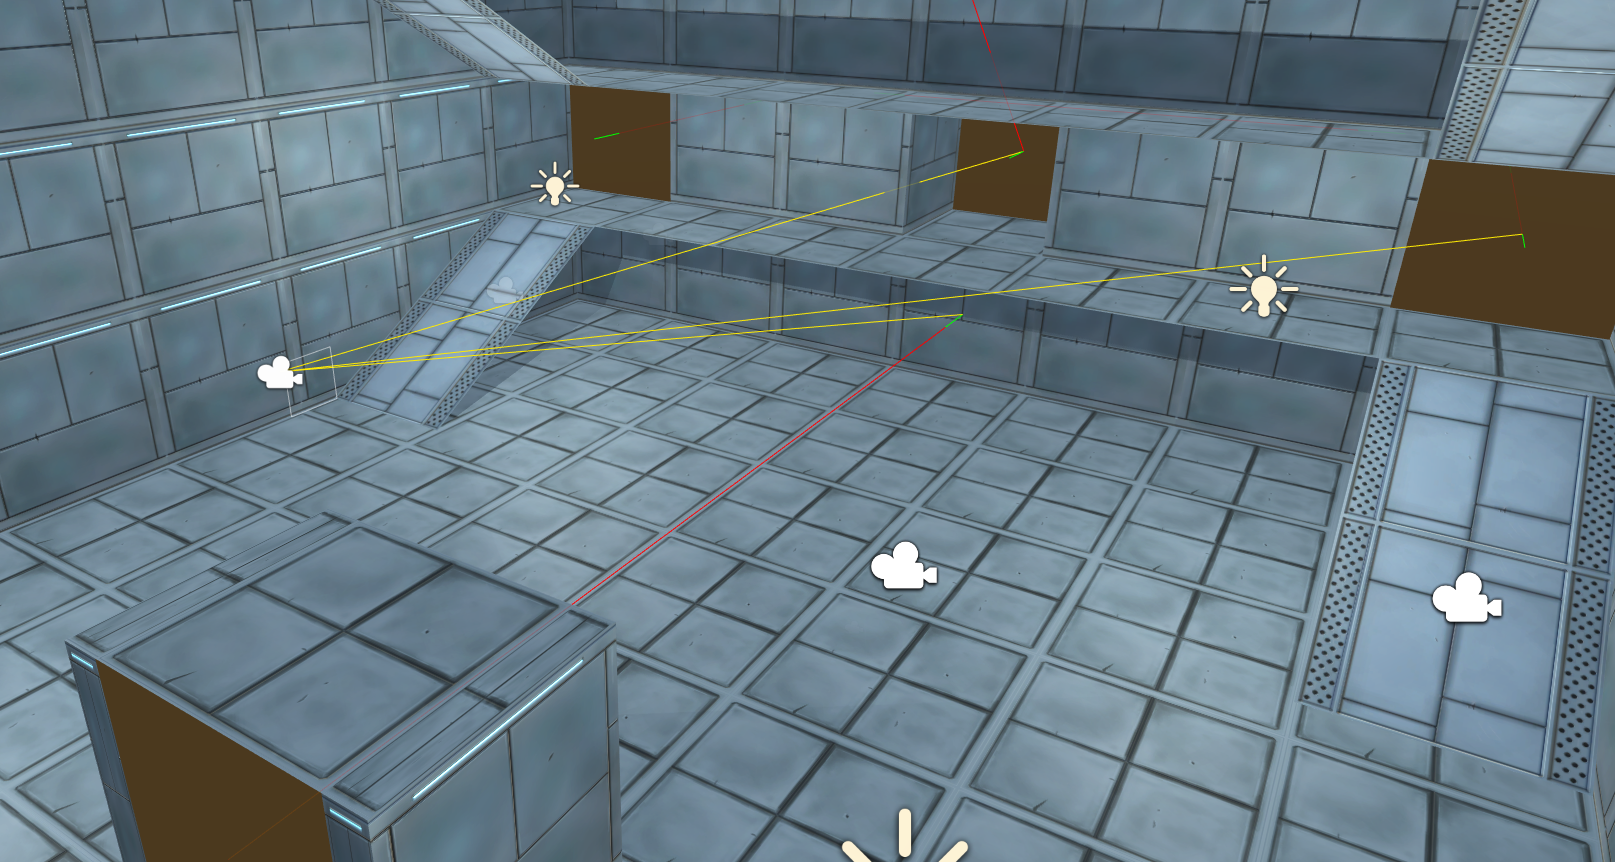
\includegraphics[width=1\textwidth]{Images/Lines_Everywhere}
			\centering
			\caption{Test scene using textured objects}
			\label{design:fig:design:tex}
		\end{figure}

		\subsubsection{Non-Euclidean Scene}

			The non-Euclidean test scene (as seen in \autoref{design:fig:design:ne}) was the first of the two scenes to be designed for the experiments.
			As a way to ensure the participants could experience a variety of the possibilities of non-Euclidean environments, a mixture of effects were chosen to be included in the scene, as labelled in \autoref{design:fig:design:ne} by the letters and corresponding red lines.

			\begin{figure}[H]
				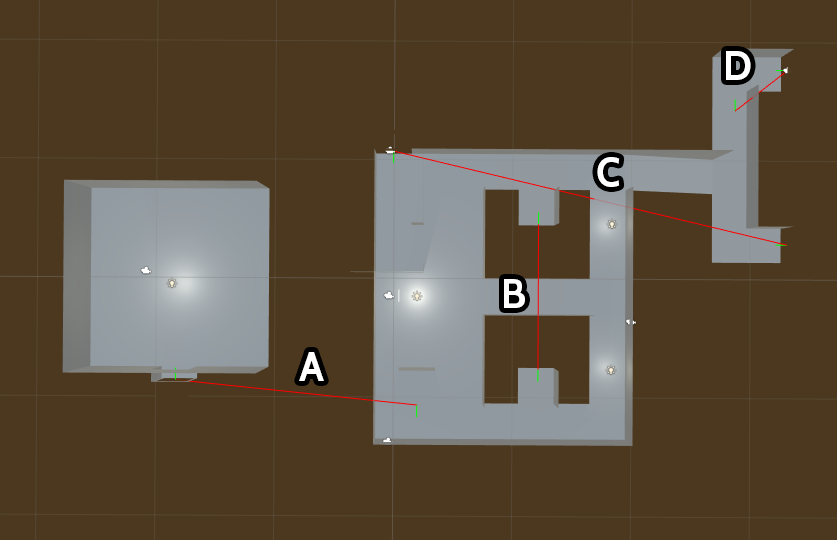
\includegraphics[width=1\textwidth]{Images/NE_Layout}
				\centering
				\caption{Labelled layout of the Non-Euclidean experiment scene}
				\label{design:fig:design:ne}
			\end{figure}

			Point \enquote{A} represents the connection shown in \autoref{design:fig:game}, which is an example of an area appearing to contain a larger area than expected from its surroundings.
			Connection \enquote{B} represents what appears to be a direct corridor to a user which both takes a shorter path than would be expected by the two parallel paths, while at the same time appears to occupy the same space as another corridor which runs perpendicular to it.
			Connection \enquote{C} appears to a user that they are able to walk directly between two completely separate areas of the room, both of which are on different levels (Note the corridor to the right of the \enquote{C} marker is a ramp leading down towards \enquote{D}).
			Finally, connection \enquote{D} gives the impression that the user is walking around a seemingly endless series of turns, however when the user turns back from where they came from, they find they have not travelled anywhere.

			The ramp connecting the two levels in the scene (As seen between points \enquote{C} and \enquote{D} in \autoref{design:fig:design:ne}) is at an angle of 20\degree, below the 21.98\degree critical angle for perceiving affordance when in VR \cite{Regia-Corte2012}.

		\subsubsection{Standard Scene}
			The standard Euclidean scene (as seen in \autoref{design:fig:design:standard}) was designed to follow a similar layout to the non-Euclidean one, or as close as could be possible with the geometric constraints.
			This decision was made to attempt to limit the factors that could affect the participant's immersion within the scenes, as a way to ensure that the results from the experiments are as consistent as possible.

			\begin{figure}[H]
				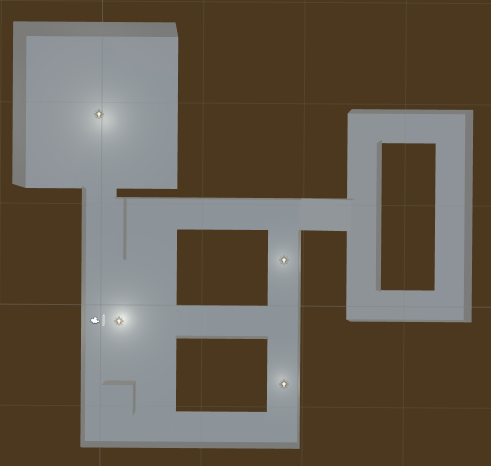
\includegraphics[width=1\textwidth]{Images/Standard_Layout}
				\centering
				\caption{Layout of the standard Euclidean experiment scene}
				\label{design:fig:design:standard}
			\end{figure}
